%%
% The BIThesis Template for Bachelor Graduation Thesis
%
% 北京理工大学毕业设计(论文)第一章节 —— 使用 XeLaTeX 编译
%
% Copyright 2020-2023 BITNP
%
% This work may be distributed and/or modified under the
% conditions of the LaTeX Project Public License, either version 1.3
% of this license or (at your option) any later version.
% The latest version of this license is in
%   http://www.latex-project.org/lppl.txt
% and version 1.3 or later is part of all distributions of LaTeX
% version 2005/12/01 or later.
%
% This work has the LPPL maintenance status `maintained'.
%
% The Current Maintainer of this work is Feng Kaiyu.
%
% 第一章节

\chapter{绪论}

\section{研究背景和意义}
% 这里插入一个参考文献,仅作参考

\subsection{三维点云配准}
21世纪以来,人工智能技术的发展对于社会有着重大的影响,智能化成为工程技术突破的内核。机器能够进行快速计算、存储和处理大量数据,并通过互联网将社会连为一体。现在由人工智能驱动的新一代机器,它们可以越来越自主地解决复杂的任务,其中以视觉为核心的机器技术快速发展,机械臂、自动驾驶、自主运动机器人等进入了人们的视野。随着2012年AlexNet\cite{krizhevsky2017imagenet} 问世以来,深度学习方法打开了计算机视觉的新大门。越来越多的深度学习方法比如VGG\cite{simonyan2014very} 、ResNet\cite{he2016deep} 、ViT\cite{dosovitskiy2020image} 被用在了图像分类、分割、场景理解等任务中。为了更好的理解真实世界,人们开始尝试将深度学习方法用于三维数据中,随着激光雷达和Kinect等高精度传感器的快速发展,点云已经成为表示三维世界的主要数据格式。2017年PointNet\cite{qi2017pointnet} 出现后,深度学习方法也同样被广泛应用在了点云处理中。

三维点云配准是点云处理中的一项基本任务\cite{qi2017pointnet,huang2021comprehensive,besl1992method} ,其在机械臂、自动驾驶、自主运动机器人等众多基于视觉方法的应用中起着关键的作用。首先是三维重建,生成完整的三维场景是各种计算机视觉应用的基础和重要技术,包括自动驾驶中的高精度三维地图重建、机器人技术中的三维环境重建等。例如,配准可以为机器人应用程序中的路线规划和决策构建三维环境。

其次,三维场景中的定位。三维场景中的定位和重定位对于机器人技术尤其重要。例如,无人驾驶汽车会估计其在地图上的位置及其与道路边界线的距离。点云配准可以将当前的实时三维视图与其所属的三维环境准确匹配,提供高精度定位服务。此应用表明,点云配准提供了机器和三维环境交互一种解决方案。

第三,位姿估计。将点云A与另一个点云B对齐可以生成与点云B相关的点云A的位姿信息。这个位姿信息可用于机器人决策。例如,点云配准可以获取环境中物体的位姿信息,以决定机械臂移动到哪里以准确抓取并移动物体。位姿估计为机器人三维环境理解提供了重要信息。

在国防安全、信息安全、环境安全等领域,无人机系统、自主导航、环境感知等技术应用愈发广泛。在这些应用中,点云配准也发挥着重要作用。例如,无人机系统需要对目标进行跟踪,而点云配准可以提供目标的位姿信息,来实现目标跟踪。点云配准可以用于环境感知,用于分割、检测、识别等任务,从而实现环境感知。在自动驾驶、机器人自主导航中,高精度的点云配准算法可以提供高精度的3D地图场景重建,为自主机器提供视觉定位、路径规划、障碍物检测等技术保障\cite{zidongjiashilujingguihua} 。


\subsection{多实例点云配准}
点云配准旨在通过对源点云和目标点云之间进行刚性变换,使得源点云和目标点云尽可能重合。点云配准的输入是两个点云,输出是一个刚性变换矩阵。点云配准的目标是找到一个刚性变换矩阵,使得源点云和目标点云之间的距离最小。传统方法中,一般流程为查找匹配点,通过SVD\cite{SVD}等方法求解出变换矩阵。随着机器学习和深度学习算法的广泛使用,基于深度学习方法和组合优化方法进一步提高了点云配准的准确率\cite{deng2018ppf,deng2018ppfnet,qin2022geometric} 。

\begin{figure*}[ht]
    \vspace{-4mm}
    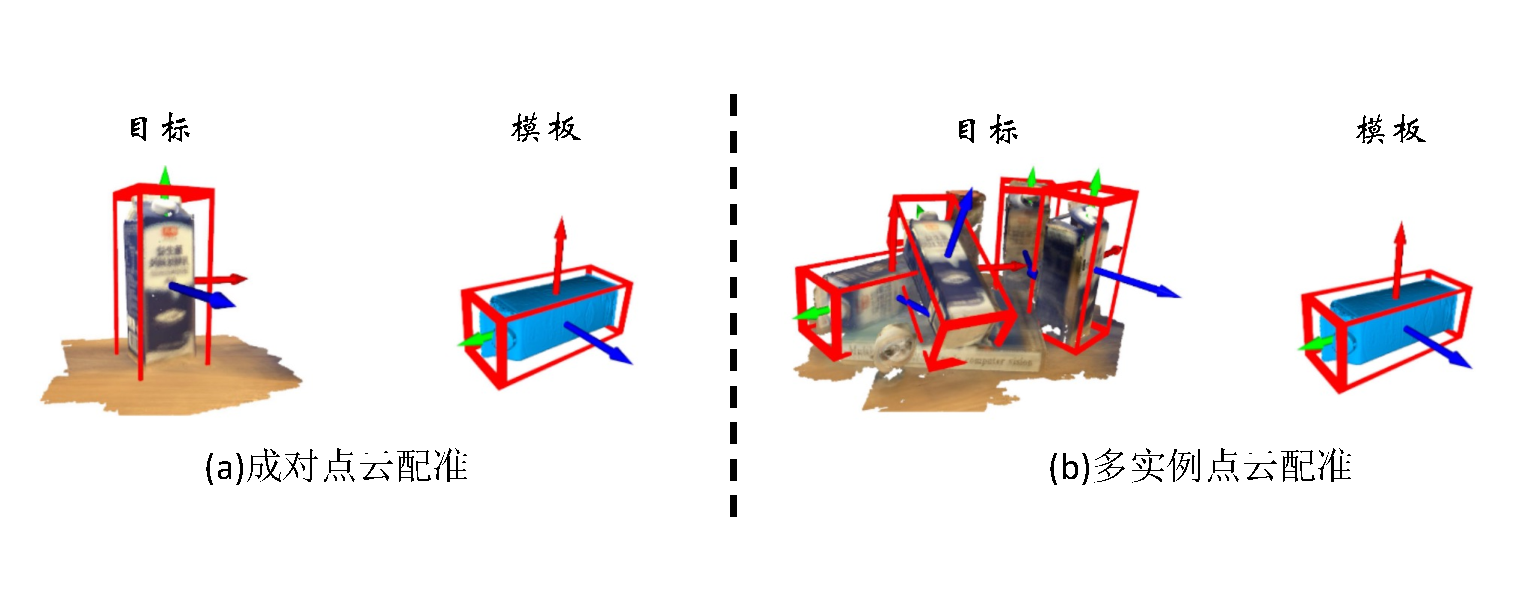
\includegraphics[width=\textwidth]{images/teaser.pdf}
    \caption{\textbf{多实例点云配准: } 给定目标的模板点云,成对点云配准(左)侧重于估计模板点云和目标点云之间的单个刚性变换,而多实例点云配准(右)旨在估计目标点云中相同物体的6D位姿。
    }
    \label{fig:teaser}
    \vspace{-10mm}
\end{figure*}

目前大多数点云配准任务研究主要集中在成对配准上。然而,在实际应用中,目标场景可能包含多个重复实例,本文需要估计模板点云与目标点云中这些重复实例之间的多个刚性变换。比如说在室内场景中,本文希望机器人能够将屋子中所有的椅子摆正,那么首先需要将多个椅子点云和模板椅子点云进行配准,求的目标椅子的位姿,通过机械运动来达到位姿改变的效果。图 \ref{fig:teaser} 展示了了一个示例。这个问题被命名为多实例点云配准,它比成对点云配准更具挑战性。针对该任务已有的现有文献研究较少,扩展现有的点云配准方法来解决这个问题并非易事。多实例点云配准不仅需要从嘈杂的对应中拒绝异常值,还需要识别单个实例的异常值集,这使得它比传统的配准问题更具挑战性。

与传统的两两配准方法相比,多实例点云配准需要解决更复杂的问题,同时也具有更广泛的应用价值。比如,在大规模场景重建任务中,通常需要处理成千上万个点云数据。单纯采用两两配准的方法可能导致累积误差,从而影响重建结果的精度。因此,研究多实例点云配准算法具有重要的实际意义。在机械臂抓取任务中,多实例点云配准算法可以在全局范围内考虑点云之间的约束关系,有助于消除局部误差和噪声的影响,从而提高配准结果的鲁棒性 \cite{stuckler2012robust} 。

尽管多实例点云配准技术在近年来取得了显著的进展,仍然存在许多亟待解决的问题。例如,现存的多实例点云配准一般采用多任务的方式,也就是先对点云分割或者三维目标检测,然后进行两两点云配准,这样的方式需要先训练点云分割或者目标检测网络,泛化性差。并且如果见到了不存在先验的点云,下游的配准任务仍然会失效。所以,本文本文会对多实例点云配准进行研究,通过点云直接进行多实例点云配准,不需要先进行点云分割或者目标检测,从而提高多实例点云配准的泛化性。


\section{国内外研究现状}

\subsection{点云配准}
点云配准长期以来一直是计算机视觉和机器人领域的一项基本任务,大致可分为直接方法 \cite{besl1992method, pomerleau2015review} 和基于特征的方法 \cite{qi2017pointnet,huang2021predator,bai2021pointdsc} 。近年来,由于深度学习的发展,许多基于特征的方法取得了最先进的性能。这些方法通常通过特征匹配产生对应关系,然后移除异常值以稳健地估计转换。尽管深度特征 \cite{qi2017pointnet,huang2021predator,bai2021pointdsc, wang2022you} 发展迅速,但特征匹配生成的对应关系仍然包含异常值。因此,去除异常点在点云配准中具有重要意义。过去,已经提出了许多传统方法来去除异常值,包括基于随机抽样一致 (Random sample consensus, RANSAC)的方法 \cite{barath2021progressive,zhao2021progressive,barath2018graph} 、基于分支和边界的方法 \cite{kluger2020consac} 以及许多其他方法 \cite{huang2021predator,yang2020teaser} 。最近,一系列基于学习的方法 \cite{bai2020d3feat,yi2018learning} 被提出,并在异常值去除方面取得了显着的效果。
以上的方法都是基于成对点云配准来完成的。然而,与成对配准不同,一个实例的内点构成多实例点云配准中所有其他实例的异常值。这种伪异常值使得很难将上述二元分类模型直接推广到多实例点云配准的情况。
现有该问题解决方案包括采用目标检测方法或对目标点云应用实例分割,将多实例点云配准问题转化为多个成对点云配准问题,但是这种方法需要预先训练一个目标检测或者点云分割网络,这样的方法对于已有点云类别是有效的,但是对于未知的类别是不适用的。另一种解决方案是通过多模型拟合,但是现有的多模型拟合方法依赖于抽样有效假设,当模型数量或离群率变高时,会涉及大量的抽样步骤,使得这些算法的效率和鲁棒性急剧下降。

\subsection{三维目标检测和实例分割}
三维物体的目标检测和实例分割与多实例点云配准有着密切的关系。输入一帧点云,目标检测模型 \cite{qi2019deep} 可以用来对获取每个目标对象的边界框,三维实例分割 \cite{wang2018sgpn,han2020occuseg} 为每个点生成实例标签。

这样的方法产生的结果类似于多实例点云配准的结果,但是它们需要将特定对象或类别的先验训练到网络中。基于点云匹配的筛选和聚类方法来进行多实例点云配准通过直接将模板点云和目标点云中的多个实例对齐来处理两组点云,而不使用任何关于输入的点云的先验信息。

\subsection{多模型拟合}
多实例配准也可以通过多模型拟合来实现,其目的是根据多个模型生成的数据点来进行建模。例如在点云中拟合多个平面 \cite{barath2018multi} ,在运动分割中估计基本矩阵 \cite{hartley1997defense} ,在多实例点云配准中计算刚性变换 \cite{tang2022multi} 等。但是由于一个实例的正常值构成所有其他实例的离群值,所以多模型拟合比单模型拟合更具挑战性。

现有的多模型拟合方法大致可以分为两类。第一类按顺序拟合模型 \cite{barath2019progressive,barath2021progressive,kanazawa2004detection,kluger2020consac} ,通过重复采样和筛选模型来进行建模。比如,Progressive-X \cite{barath2019progressive} 和Progressive-X+ \cite{barath2021progressive} 使用了表现更好的Graph-cut RANSAC \cite{barath2018graph} 作为采样方法来生成假设。CONSAC \cite{kluger2020consac} 首次将深度模型引入多模型拟合中,使用类似PointNet \cite{qi2017pointnet} 的网络来引导采样。通过重复采样来恢复单个实例,从输入中删除异常值,以顺序的方式来检测实例。

第二类模型同时拟合多个模型 \cite{tang2022multi,toldo2008robust,magri2016multiple,magri2014t,magri2015robust} 。许多基于偏好分析的方法 \cite{toldo2008robust,magri2015robust} 最初对一系列假设进行采样,然后根据假设的残差对输入点进行聚类。之前的工作 \cite{tang2022multi} 利用点云刚性变换空间一致性 \cite{leordeanu2005spectral} 和以自下而上的方式基于距离不变矩阵对对应关系进行聚类。\\
% 本项目希望基于旋转等变的描述子来实现性能的初步提升,希望在模型中加入更多的内在形状和几何信息。通过端到端的方法优化整个方法系统,实现更高的准确性和鲁棒性。
\section{论文结构安排}
本论文共分为6章。

第一章为绪论,本章主要阐述了三维点云配准研究的重要性、背景以及现有的研究进展。通过对国内外三维点云配准研究文献的梳理和调查,本文对该领域的发展轨迹和现状进行了总结,并分析了先前研究所展现出的优点与缺点。同时,本文也详细介绍了本研究所完成的主要任务和做出的关键贡献。考虑到过去的研究中仍存在未完全解决的问题和挑战,本文特别指出了本研究所应用的策略和解决方案。最后,本文规划了清晰的文章结构,以引导读者理解本研究的整体框架。

在第二章,本文主要阐述了三维点云的基本数据格式和在本研究中所涉及的基础数学知识。同时,本文对在本研究中所用到的关于三维刚体变换的基础知识进行了详尽的总结和描述。

第三章在介绍了主要的数据集和评价指标后,引出深度学习方法在三维点云配准领域的研究与应用,并结合深度学习在三维点云配准领域做出的代表性工作 PointNet \cite{qi2017pointnet} 和 PointNet++ \cite{qi2017pointnet++} 进行介绍,并介绍和使用 PREDATOR \cite{huang2021predator} 作为骨干网络提取点云的点对特征供后续使用。

第四章主要介绍了本文提出的多实例点云配准,首先本文根据点云的特征进行聚类,然后对每个聚类进行对应聚类,最后进行刚性变换估计;其次,本文引入深度学习的方法,学习鲁棒的点对特征,进行谱聚类,得到了点云配准更好的效果和更高的指标。

第五章主要介绍了本文的实验结果,包括多实例点云配准的定性和定量实验,证明了本文提出的方法的有效性和鲁棒性。
\section{小结}
本章主要介绍了点云配准任务以及多实例点云配准任务的研究背景和研究意义、国内外研究现状。然后介绍了本文的研究内容和结构安排。
